\RequirePackage{luatex85}
\documentclass[tikz]{standalone}
\usepackage{amsmath}
\begin{document}
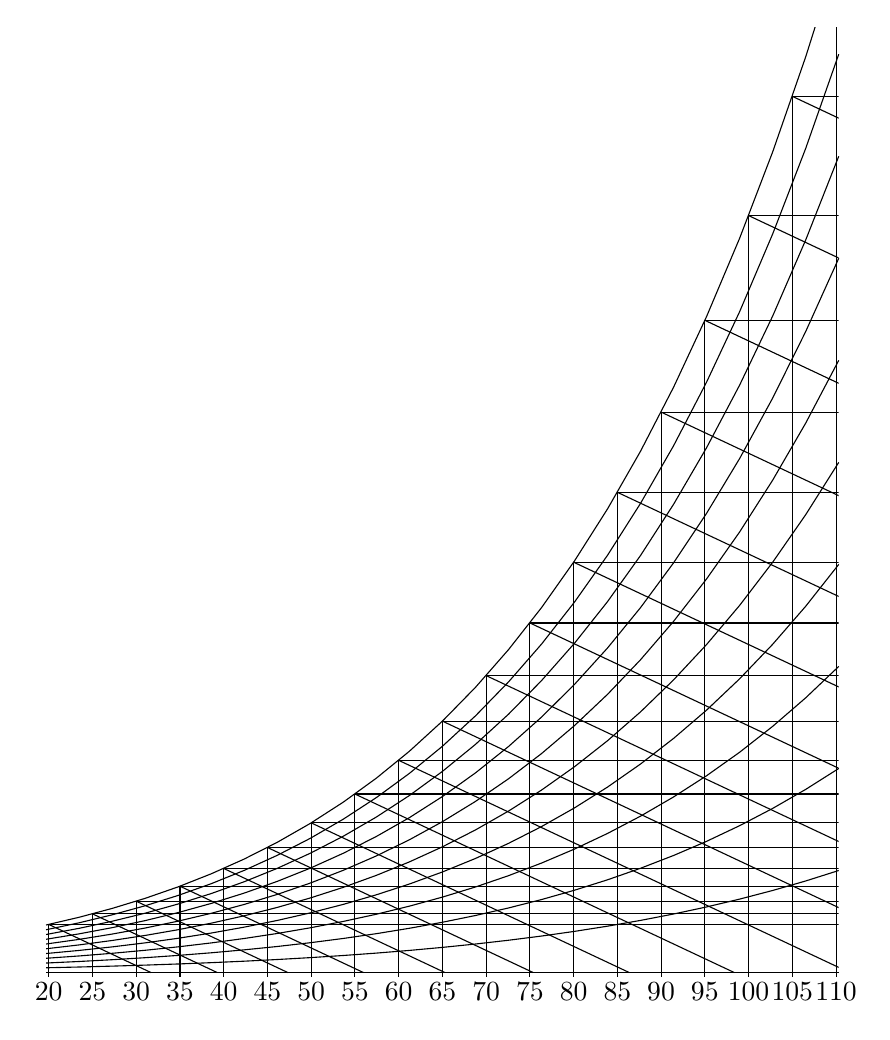
\begin{tikzpicture}[domain=19.7:110.3, scale=0.2]
\clip (265,-2.5) rectangle (318,60);
\foreach \y in {1,...,10} \draw
	plot ({(\x-32)/1.8+273}, 
		{0.1*\y*exp(20.386-5132/((\x-32)/1.8+273))});
\draw ({(19.7-32)/1.8+273},0) 
	-- ({(110.3-32)/1.8+273},0);
\foreach \x in {20,25,...,110} \draw
	({(\x-32)/1.8+273},0) node[below] {\x};
\clip ({(19.7-32)/1.8+273},-0.3) rectangle 
	({(110.3-32)/1.8+273},
		{exp(20.386-5132/((110.3-32)/1.8+273))});
\foreach \x in {20,25,...,110} \draw
	({(\x-32)/1.8+273},
		{exp(20.386-5132/((\x-32)/1.8+273))})
	edge[-] ({(110.3-32)/1.8+273)},
		{exp(20.386-5132/((\x-32)/1.8+273))})
	edge[-] ({(\x-32)/1.8+273
		+2.125*exp(20.386-5132/((\x-32)/1.8+273)))},0)
	edge[-] ({(\x-32)/1.8+273)},-0.3)
	;
\end{tikzpicture}

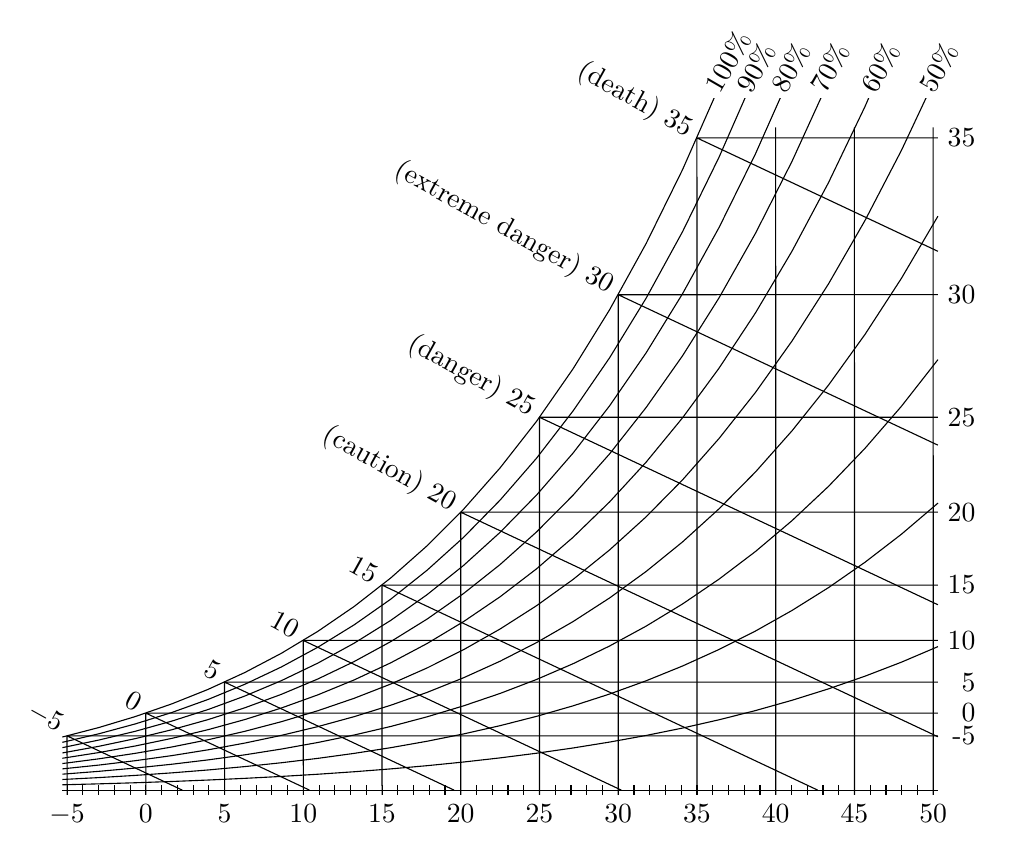
\begin{tikzpicture}[scale=0.2,
	declare function={f(\x)=exp(20.386-5132/\x);}]
\def\a{267.7}
\def\b{323.3}
\clip (\a - 2.2, -2.5) rectangle (\b+3.2, {f(35+273)+7});
\draw (\a, -0.3) grid (\b, 0.3);
%\clip (\a - 2.2, -2.5) rectangle (\b+3.2, {f(35+273)});
\foreach \x in {-5, 0, ..., 35} \draw
	(\x + 273, {f(\x + 273)}) coordinate (a)
	(a) -- (\b, {f(\x + 273)}) node[right] {$\quad\llap\x$}
	(a) node[above left, rotate=-29, yshift=-5] {$\x$}
	-- ++({min(2.125*f(\x+273), \b-\x-273)}, 
		{max(-8/17*(\b-\x-273), -f(\x+273))})
	(a) -- (\x + 273, -0.3) node[below] {$\x$}
	;
\foreach \x in {40, 45, ..., 50} \draw
	(\x + 273, {f(35.3+273)}) coordinate (a)
	(a) -- (\x + 273, -0.3) node[below] {$\x$}
	;
\foreach \x/\n in {20/caution, 25/danger, 30/extreme danger, 35/death} \draw
	(\x + 273, {f(\x+273)})
	node[above left, rotate=-29, yshift=-5] {\smash{(\n)}$\quad\,\,$}
	;
\foreach \h/\x in {100/0.6, 90/2.6, 80/4.8, 70/7.3, 60/10.5, 50/14.2} \draw
	(35+273+\x, {f(35+273)+2.5}) node[above, rotate=60, right] {$\h\%$};
\clip (\a - 2.2, -2.5) rectangle (\b+3.2, {f(35+273)+2.5});
\foreach \y in {1, ..., 10} \draw
	plot[domain=\a:\b] (\x, {f(\x)*\y/10});
\end{tikzpicture}

%\begin{tikzpicture}[domain=272.7:313.3, scale=0.2]
%\foreach \y in {1,...,10} \draw
%	plot (\x, {0.1*\y*exp(20.386-5132/\x)});
%\draw ({273-0.3},-0.3) grid ({273+40+0.3},+0.3);
%\foreach \x in {0,2,...,40} \draw
%	(\x+273,0) node[below] {\x};
%\clip (272.7,0) rectangle 
%	(313.3,{exp(20.386-5132/313.3)});
%\foreach \x in {0,...,40} \draw
%	(\x+273,{exp(20.386-5132/(\x+273))})
%	edge[-] (313+0.3,{exp(20.386-5132/(\x+273))})
%	edge[-] ({\x+273+2.125*exp(20.386-5132/(\x+273))},0)
%	edge[-] (\x+273,-0.3)
%	;
%\end{tikzpicture}
\end{document}

2.125=(40-14)/exp(20.386-5132/(273+14))

C*1.8 +32 = F
C = (F-32)/1.8+273